% Demo: the round-2 figures in a REVTeX two-column paper (10 pt, \columnwidth = 246pt, \textwidth = 510pt)
\documentclass[aps,prl,twocolumn,10pt,nofootinbib]{revtex4-2}
\usepackage[T1]{fontenc}
\usepackage{lmodern}
\usepackage{graphicx,amsmath,amssymb,tikz,contour}
\graphicspath{{../out/}}
\def\cmwdir{../out/}
\begin{document}
\title{Prototype figures from the new export (round 2)}
\author{Complex Map Workbench}
\maketitle
The Cayley transform $F(z)=(z-i)/(z+i)$ takes the upper half-plane $\mathbb{H}$ onto the unit disk $\mathbb{D}$; it sends $i$ to the center and the point at infinity to $1$. Every figure here is placed at its natural size: tick labels are \verb|\footnotesize| and panel labels \verb|\small| of this 10\,pt text, set in the same Latin Modern as this paragraph. Lines are vector strokes of at least 0.5\,pt; only the shading is an image (flat tones at 600\,dpi in indexed color, continuous tone at 300\,dpi), and no file declares a font or uses transparency.

% cayley.pdf is made for \columnwidth = 246pt; include it unscaled so its labels match your text.
% If your \columnwidth is narrower, use [width=\columnwidth] (the labels will shrink). Preamble: \usepackage{graphicx,amsmath,amssymb}
\begin{figure}[tbp]
  \centering
  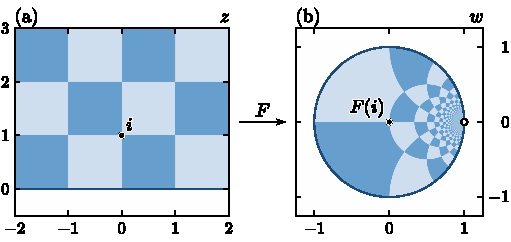
\includegraphics{cayley}
  \caption{(a) The upper half-plane $\operatorname{Im} z>0$ with the point $i$. (b) Its image under $F(z)=(z-i)/(z+i)$, the unit disk, with $F(i)=0$. A checkerboard of unit cells in the $z$-plane is carried by $F$; the point at infinity goes to $1$ (open circle).}
  \label{fig:cayley}
\end{figure}

Figure~\ref{fig:cayley} is the column preset. Every figure here is placed at its natural size: tick labels are \verb|\footnotesize| and panel labels \verb|\small| of this 10\,pt text, set in the same Latin Modern as this paragraph. Lines are vector strokes of at least 0.5\,pt; only the shading is an image (flat tones at 600\,dpi in indexed color, continuous tone at 300\,dpi), and no file declares a font or uses transparency.

% cayley-wide.pdf is made for \textwidth = 510pt; include it unscaled so its labels match your text.
% If your \textwidth is narrower, use [width=\textwidth] (the labels will shrink). Preamble: \usepackage{graphicx,amsmath,amssymb}
\begin{figure*}[tbp]
  \centering
  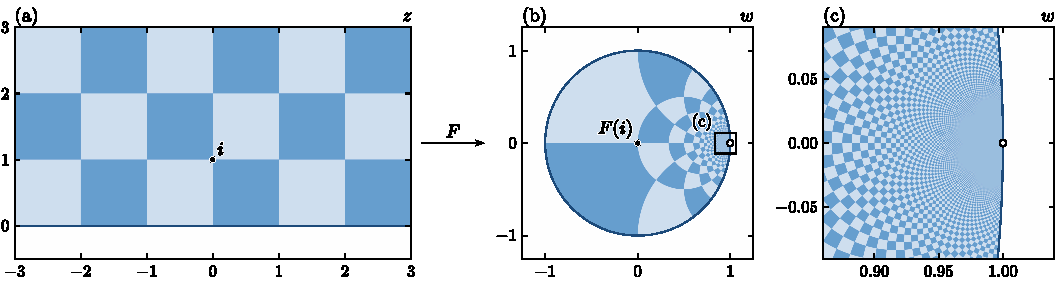
\includegraphics{cayley-wide}
  \caption{(a) The upper half-plane $\operatorname{Im} z>0$ with the point $i$. (b) Its image under $F(z)=(z-i)/(z+i)$, the unit disk, with $F(i)=0$; the point at infinity goes to $1$ (open circle). (c) Detail of (b) near $w=1$, where the image cells accumulate. Shading: a checkerboard of unit cells in the $z$-plane and its image.}
  \label{fig:cayley-wide}
\end{figure*}
% cayley-deformation.pdf is made for \textwidth = 510pt; include it unscaled so its labels match your text.
% If your \textwidth is narrower, use [width=\textwidth] (the labels will shrink). Preamble: \usepackage{graphicx,amsmath,amssymb}
\begin{figure*}[tbp]
  \centering
  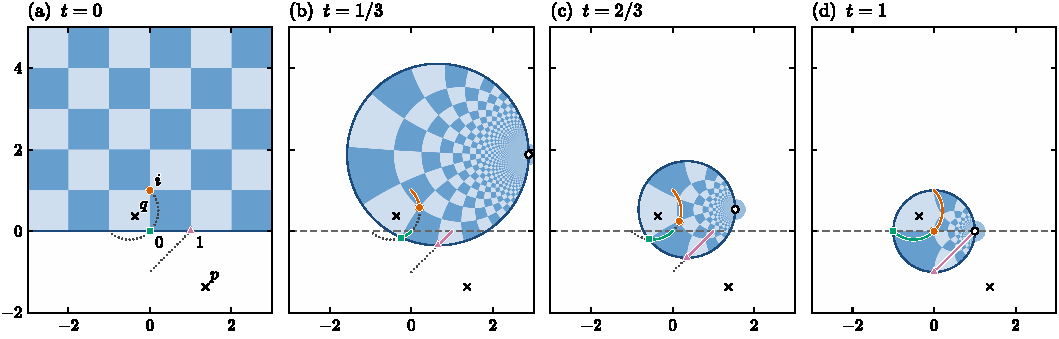
\includegraphics{cayley-deformation}
  \caption{The Cayley map as a deformation: $H_t(\mathbb{H})$ at (a) $t=0$, (b) $t=1/3$, (c) $t=2/3$ and (d) $t=1$, where $H_t$ is the elliptic M\"obius map fixing $p=\tfrac{1+\sqrt3}{2}(1-i)$ and $q=\tfrac{1-\sqrt3}{2}(1-i)$ with $H_t'(p)=e^{2\pi i t/3}$, so $H_0=\mathrm{id}$ and $H_1=F$. Solid: the paths $t\mapsto H_t(z)$ of $z=i$ (circle), $0$ (square) and $1$ (triangle) up to the frame's $t$; dotted: the rest of each path; dashed: the real axis; open circle: $H_t(\infty)$.}
  \label{fig:cayley-deformation}
\end{figure*}

Figure~\ref{fig:cayley-wide} is the full-width preset with a detail panel, and Fig.~\ref{fig:cayley-deformation} prints the deformation as a filmstrip whose panels can be cited, e.g.\ Fig.~\ref{fig:cayley-deformation}(b). Every figure here is placed at its natural size: tick labels are \verb|\footnotesize| and panel labels \verb|\small| of this 10\,pt text, set in the same Latin Modern as this paragraph. Lines are vector strokes of at least 0.5\,pt; only the shading is an image (flat tones at 600\,dpi in indexed color, continuous tone at 300\,dpi), and no file declares a font or uses transparency.

% cayley-bw.pdf is made for \columnwidth = 246pt; include it unscaled so its labels match your text.
% If your \columnwidth is narrower, use [width=\columnwidth] (the labels will shrink). Preamble: \usepackage{graphicx,amsmath,amssymb}
\begin{figure}[tbp]
  \centering
  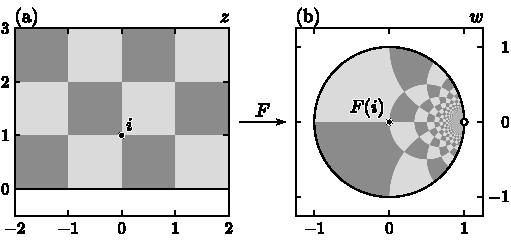
\includegraphics{cayley-bw}
  \caption{(a) The upper half-plane $\operatorname{Im} z>0$ with the point $i$. (b) Its image under $F(z)=(z-i)/(z+i)$, the unit disk, with $F(i)=0$. A checkerboard of unit cells in the $z$-plane is carried by $F$; the point at infinity goes to $1$ (open circle).}
  \label{fig:cayley-bw}
\end{figure}

Figure~\ref{fig:cayley-bw} is the black-and-white version: 8-bit gray images, 45\,\% and 14\,\% gray. Every figure here is placed at its natural size: tick labels are \verb|\footnotesize| and panel labels \verb|\small| of this 10\,pt text, set in the same Latin Modern as this paragraph. Lines are vector strokes of at least 0.5\,pt; only the shading is an image (flat tones at 600\,dpi in indexed color, continuous tone at 300\,dpi), and no file declares a font or uses transparency.

% phase.pdf is made for \columnwidth = 246pt; include it unscaled so its labels match your text.
% If your \columnwidth is narrower, use [width=\columnwidth] (the labels will shrink). Preamble: \usepackage{graphicx,amsmath,amssymb}
\begin{figure}[tbp]
  \centering
  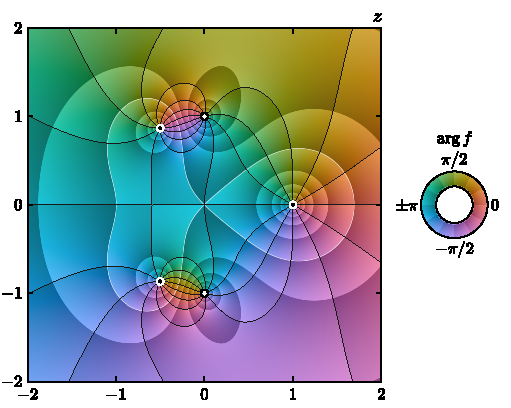
\includegraphics{phase}
  \caption{Phase portrait of $f(z)=(z^3-1)/(z^2+1)$ on $[-2,2]^2$: the color shows $\arg f(z)$ (key at right) and the thin lines are the level sets $\arg f\in\frac{\pi}{6}\mathbb{Z}$. Zeros (dots) at the cube roots of unity; simple poles (open circles) at $\pm i$.}
  \label{fig:phase}
\end{figure}
% phase-bw.pdf is made for \columnwidth = 246pt; include it unscaled so its labels match your text.
% If your \columnwidth is narrower, use [width=\columnwidth] (the labels will shrink). Preamble: \usepackage{graphicx,amsmath,amssymb}
\begin{figure}[tbp]
  \centering
  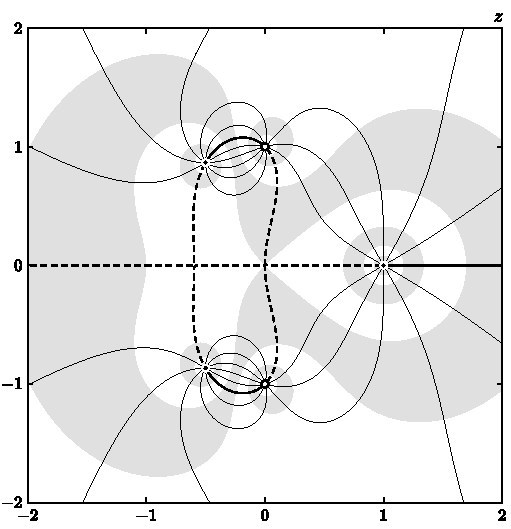
\includegraphics{phase-bw}
  \caption{Phase portrait of $f(z)=(z^3-1)/(z^2+1)$ on $[-2,2]^2$ as level sets of $\arg f$ at multiples of $\pi/6$; heavy: $\arg f=0$, dashed: $\arg f=\pi$. Bands: $\lfloor\log_2|f|\rfloor$ even (gray) or odd (white). Zeros (dots) at the cube roots of unity; simple poles (open circles) at $\pm i$.}
  \label{fig:phase-bw}
\end{figure}

Figures~\ref{fig:phase} and~\ref{fig:phase-bw} are the Phase view in color and in black and white. Every figure here is placed at its natural size: tick labels are \verb|\footnotesize| and panel labels \verb|\small| of this 10\,pt text, set in the same Latin Modern as this paragraph. Lines are vector strokes of at least 0.5\,pt; only the shading is an image (flat tones at 600\,dpi in indexed color, continuous tone at 300\,dpi), and no file declares a font or uses transparency.

\begin{figure}[tbp]
  \centering
  % cayley: labels typeset by your document, over cayley-art.pdf. Made for \columnwidth = 246pt.
% Needs \usepackage{tikz,graphicx,amsmath,contour}. If the art lives in a folder, \def\cmwdir{figs/} first.
\providecommand\cmwdir{}
\begin{tikzpicture}[x=1bp,y=1bp,inner sep=0pt,outer sep=0pt]
  \useasboundingbox (0,0) rectangle (245.08,115.95);
  \node[anchor=south west] at (0,0) {\includegraphics{\cmwdir cayley-art.pdf}};
  \node[anchor=north,font=\footnotesize] at (7.00,9.40) {$-2$};
  \node[anchor=north,font=\footnotesize] at (32.71,9.40) {$-1$};
  \node[anchor=north,font=\footnotesize] at (58.43,9.40) {$0$};
  \node[anchor=north,font=\footnotesize] at (84.14,9.40) {$1$};
  \node[anchor=north,font=\footnotesize] at (109.86,9.40) {$2$};
  \node[anchor=east,font=\footnotesize] at (4.50,25.46) {$0$};
  \node[anchor=east,font=\footnotesize] at (4.50,51.17) {$1$};
  \node[anchor=east,font=\footnotesize] at (4.50,76.89) {$2$};
  \node[anchor=east,font=\footnotesize] at (4.50,102.60) {$3$};
  \node[anchor=south west,font=\small] at (60.60,53.35) {\contour{white}{$i$}};
  \node[anchor=north,font=\footnotesize] at (150.86,9.40) {$-1$};
  \node[anchor=north,font=\footnotesize] at (186.86,9.40) {$0$};
  \node[anchor=north,font=\footnotesize] at (222.86,9.40) {$1$};
  \node[anchor=east,font=\footnotesize] at (244.58,21.60) {$-1$};
  \node[anchor=east,font=\footnotesize] at (244.58,57.60) {$0$};
  \node[anchor=east,font=\footnotesize] at (244.58,93.60) {$1$};
  \node[anchor=south east,font=\small] at (184.68,59.78) {\contour{white}{$F(i)$}};
  \node[anchor=base west,font=\small] at (7.00,105.60) {(a)};
  \node[anchor=base east,font=\small] at (109.86,105.60) {$z$};
  \node[anchor=base west,font=\small] at (141.86,105.60) {(b)};
  \node[anchor=base east,font=\small] at (231.86,105.60) {$w$};
  \node[anchor=south,font=\small] at (125.86,60.20) {$F$};
\end{tikzpicture}

  \caption{The overlay format: the art of Fig.~\ref{fig:cayley} with every label typeset by this document. (a) The upper half-plane $\operatorname{Im} z>0$ with the point $i$. (b) Its image under $F(z)=(z-i)/(z+i)$, the unit disk, with $F(i)=0$. A checkerboard of unit cells in the $z$-plane is carried by $F$; the point at infinity goes to $1$ (open circle).}
  \label{fig:overlay}
\end{figure}
Figure~\ref{fig:overlay} uses the overlay. Every figure here is placed at its natural size: tick labels are \verb|\footnotesize| and panel labels \verb|\small| of this 10\,pt text, set in the same Latin Modern as this paragraph. Lines are vector strokes of at least 0.5\,pt; only the shading is an image (flat tones at 600\,dpi in indexed color, continuous tone at 300\,dpi), and no file declares a font or uses transparency.

\end{document}
